\chapter[Basic Concepts]{Basic Concepts of Probability}

The theory of probability provides the mathematical tools necessary to study and analyze uncertain phenomena that occur in nature.
It establishes a formal framework to understand and predict the outcome of a random experiment.
It can also be used to model complex systems and characterize stochastic processes.
This is instrumental in designing efficient solutions to many engineering problems.
Two components define a probabilistic model, a sample space and a probability law.


\section{Sample Spaces and Events}

In the context of probability theory, an \emph{experiment} is a random process that produces one of several \emph{outcomes}. \index{Experiment} \index{Outcome}
The set of all possible outcomes is called the \emph{sample space} of the experiment, and it is denoted by $\Omega$. \index{Sample space}
An \emph{admissible} subset of the sample space is called an \emph{event}. \index{Event}

\begin{center}
\begin{psfrags}
\psfrag{1}[c]{$1$}
\psfrag{2}[c]{$2$}
\psfrag{3}[c]{$3$}
\psfrag{4}[c]{$4$}
\psfrag{5}[c]{$5$}
\psfrag{6}[c]{$6$}
\psfrag{7}[c]{$7$}
\psfrag{S}[l]{Sample Space $\Omega$}
\psfrag{E}[l]{One Event}
\psfrag{O}[r]{One Outcome}
\includegraphics[height=4.85cm]{Figures/2Chapter/samplespace}
\end{psfrags}
\end{center}

\begin{example}
The rolling of a die forms a common experiment.
The sample space $\Omega$ corresponding to this experiment is given by the six faces of a die.
The set of prime numbers less than or equal to six, namely $\{ 2, 3, 5 \}$, is one of many possible events.
The actual number observed after rolling the die is the outcome of the experiment.

\begin{center}
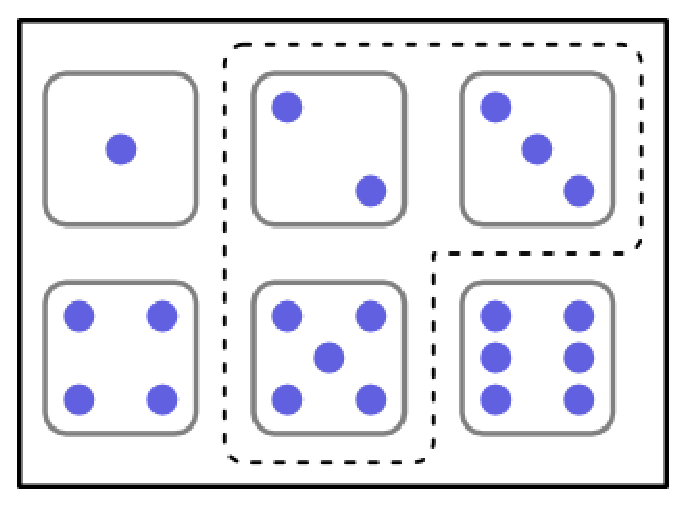
\includegraphics[height=3.375cm]{Figures/2Chapter/dices}
\end{center}
\end{example}

There is essentially no restriction on what constitutes an experiment.
The flipping of a coin, the flipping of $n$ coins, and the flipping of an infinite sequence of coins are all random experiments.
Also, two similar experiments may have different sample spaces.
The sample space $\Omega$ for observing the number of heads in $n$ tosses of a coin is $\{ 0, 1, \ldots, n \}$; whereas for describing the complete history of the $n$ coin tosses, the sample space becomes much larger with $2^n$ distinct sequences of heads and tales.
Ultimately, the choice of a particular sample space depends on the properties one wishes to observe.
Yet some rules must be followed in selecting a sample space.
\begin{enumerate}
\item The elements of a sample space should be \emph{distinct} and \emph{mutually exclusive}. \index{Distinct elements} \index{Mutually exclusive}
This insures that the outcome of an experiment is unique.
\item A sample space must be \emph{collectively exhaustive}. \index{Collectively exhaustive}
That is, every possible outcome of the experiment must be accounted for in the sample space.
\end{enumerate}
The sample space should be detailed enough to distinguish between all outcomes of interest, while avoiding frivolous details.

\begin{example}
Consider the space composed of the odd integers contained between one and six, the even integers contained between one and six, and the prime numbers less than or equal to six.
This space cannot be a sample space for the rolling of a die since its elements are not mutually exclusive.
In particular, the numbers three and five are both odd and prime, while the number two is prime and even.
This violates the uniqueness criterion.

\begin{center}
\includegraphics[height=4.125cm]{Figures/2Chapter/nonadmissiblespace}
\end{center}

Alternatively, the elements of the space composed of the odd numbers between one and six, and the even numbers between one and six, are distinct and mutually exclusive;
an integer cannot be simultaneously even and odd.
Furthermore, this space is collectively exhaustive since every integer between one and six is either even or odd.
This latter space is a possible sample space for the rolling of a die.

\begin{center}
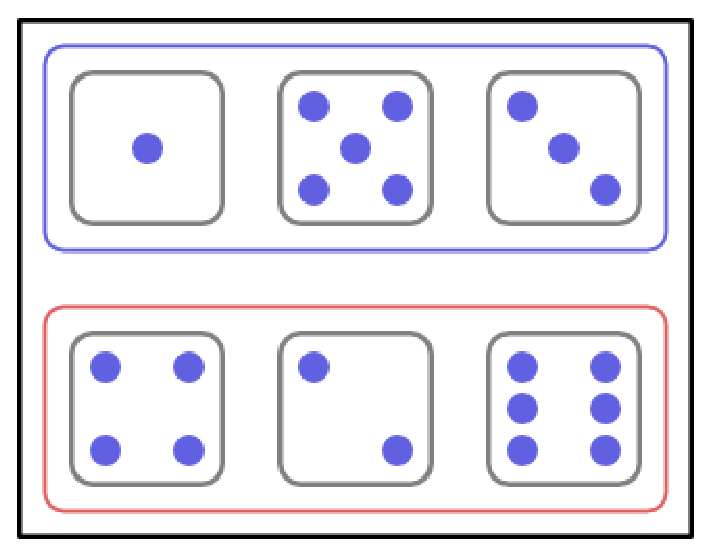
\includegraphics[height=3.75cm]{Figures/2Chapter/admissiblespace}
\end{center}
\end{example}


\section{Probability Laws}
\label{section:ProbabilityLaws}

A \emph{probability law} specifies the likelihood of any event related to an experiment. \index{Probability law}
Formally, a probability law assigns to every event $A$ a number $\Pr (A)$, called the \emph{probability of event $A$}, such that the following axioms are satisfied.
\begin{enumerate}
\item \textbf{(Nonnegativity)} $\Pr (A) \geq 0$, for every event $A$.
\item \textbf{(Normalization)} The probability of the sample space $\Omega$ is equal to one,
\begin{equation*}
\Pr (\Omega) = 1 .
\end{equation*}
\item \textbf{(Countable Additivity)} If $A$ and $B$ are disjoint events with $A \cap B = \emptyset$, then the probability of their union satisfies
\begin{equation*}
\Pr (A \cup B) = \Pr (A) + \Pr (B) .
\end{equation*}
More generally, if $A_1, A_2, \ldots$ is a sequence of disjoint events and $\bigcup_{k=1}^{\infty} A_k$ is itself an admissible event then
\begin{equation*}
\Pr \left( \bigcup_{k=1}^{\infty} A_k \right)
= \sum_{k = 1}^{\infty} \Pr (A_k) .
\end{equation*}
\end{enumerate}

A number of properties can be deduced from the three axioms of probability.
We prove two such properties below.
The first property describes the relation between inclusion and probabilities.
\begin{proposition}
If $A \subset B$, then $\Pr (A) \leq \Pr (B)$.
\end{proposition}
Since $A \subset B$, we have $B = A \cup (B - A)$.
Noting that $A$ and $B - A$ are disjoint sets, we get
\begin{equation*}
\Pr (B) = \Pr (A) + \Pr (B - A) \geq \Pr (A) ,
\end{equation*}
where the inequality follows from the nonnegativity of probability laws.

\begin{center}
\begin{psfrags}
\psfrag{A}[c]{$A$}
\psfrag{B}[l]{$B$}
\psfrag{D}[l]{$B - A$}
\includegraphics[height=3.03cm]{Figures/2Chapter/subset}
\end{psfrags}
\end{center}

The second property specifies the probability of the union of two events that are not necessarily mutually exclusive.
\begin{proposition}
$\Pr (A \cup B) = \Pr (A) + \Pr (B) - \Pr (A \cap B)$.
\end{proposition}

Using the third axiom of probability on the disjoint sets $A$ and $(A \cup B) - A$, we can write
\begin{equation*}
\Pr (A \cup B)
= \Pr (A) + \Pr ((A \cup B) - A)
= \Pr (A) + \Pr (B - A) .
\end{equation*}
Similarly, applying the third axiom to $A \cap B$ and $B - (A \cap B)$, we obtain
\begin{equation*}
\Pr (B)
= \Pr (A \cap B) + \Pr (B - (A \cap B))
= \Pr (A \cap B) + \Pr (B - A) .
\end{equation*}
Combining these two equations yields the desired result.

\begin{center}
\begin{psfrags}
\psfrag{A}[r]{$A$}
\psfrag{B}[l]{$B$}
\psfrag{I}[c]{$A \cap B$}
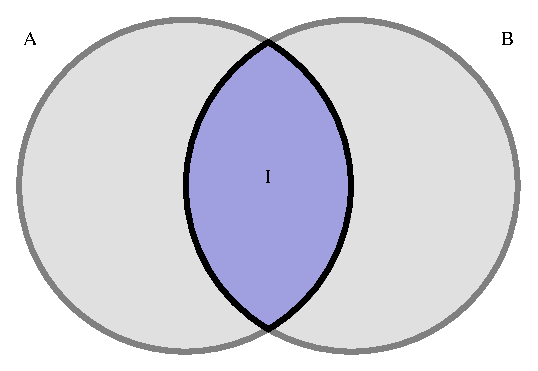
\includegraphics[height=3.03cm]{Figures/2Chapter/intersection}
\end{psfrags}
\end{center}


\subsection{Finite Sample Spaces}
\label{section:FiniteSampleSpaces}

If a sample space $\Omega$ contains a finite number of elements, then a probability law on $\Omega$ is determined completely by the probabilities of individual outcomes.
Denote a sample space $\Omega$ containing $n$ elements by $\Omega = \{ s_1, s_2, \ldots, s_n \}$.
Any event in $\Omega$ is of the form $A = \{ s_i \in \Omega | i \in \IndexSet \}$, where $\IndexSet$ is a subset of the integers one through $n$.
The probability of event $A$ is therefore given by the third axiom of probability,
\begin{equation*}
\Pr (A)
= \Pr ( \{ s_i \in \Omega | i \in \IndexSet \} )
= \sum_{i \in \IndexSet} \Pr (s_i) .
\end{equation*}
Note that, by definition, distinct outcomes are always disjoint events.

If in addition all the elements of $\Omega$ are equally likely with
\begin{equation*}
\Pr (s_1) = \Pr (s_2) = \cdots = \Pr (s_n) = \frac{1}{n} ,
\end{equation*}
then the probability of an event $A$ becomes
\begin{equation} \label{equation:ProbEquiProbableOutcomes}
\Pr (A) = \frac{ |A| }{n}
= \frac{ \text{number of elements in $A$} }{n} .
\end{equation}

\begin{example}
The rolling of a fair die is an experiment with a finite number of equally likely outcomes.
The probability of observing any of the faces labeled one through six is $1/6$.
The probability of any event can easily be computed by counting the number of distinct outcomes included in the event.
For instance, the probability of rolling a prime number is
\begin{equation*}
\Pr (\text{outcome is prime})
= \Pr ( \{ 2, 3, 5 \} )
= \Pr (2) + \Pr(3) + \Pr(5) = \frac{3}{6} .
\end{equation*}
\end{example}


\subsection{Countably Infinite Models}

Consider a sample space that consists of a countably infinite number of elements, $\Omega = \{ s_1, s_2, \ldots \}$.
Again, a probability law on $\Omega$ is specified by the probabilities of individual outcomes.
An event in $\Omega$ can be written as $A = \{ s_j \in \Omega | j \in \JndexSet \}$, where $\JndexSet$ is a subset of the positive integers.
Using the third axiom of probability, $\Pr (A)$ is given by
\begin{equation*}
\Pr (A)
= \Pr ( \{ s_j \in \Omega | j \in \JndexSet \} )
= \sum_{j \in \JndexSet} \Pr (s_j) .
\end{equation*}
The possibly infinite sum $\sum_{j \in \JndexSet} \Pr (s_j)$ always converges since the summands are nonnegative and the sum is bounded above by one.
It is therefore well-defined.

\begin{example} \label{example:CoinTossSequence}
Suppose that a fair coin is tossed repetitively until heads is observed.
The number of coin tosses is recorded as the outcome of this experiment.
The sample space for this experiment is $\Omega = \{ 1, 2, \ldots \}$, a countably infinite set.

\begin{center}
\begin{psfrags}
\psfrag{1}[c]{$1$}
\psfrag{2}[c]{$2$}
\psfrag{3}[c]{$3$}
\psfrag{4}[c]{$4$}
\psfrag{5}[c]{$5$}
\psfrag{6}[c]{$6$}
\psfrag{7}[c]{$7$}

\includegraphics[height=0.765cm]{Figures/2Chapter/countablespace}
\end{psfrags}
\end{center}

The probability of observing heads on the first trial is $0.5$, and the probability of observing heads for the first time on trial $k$ is $2^{-k}$.
The probability of the entire sample space is equal to
\begin{equation*}
\Pr ( \Omega ) = \sum_{k=1}^{\infty} \Pr (k)
= \sum_{k=1}^{\infty} \frac{1}{2^k} = 1 ,
\end{equation*}
as expected.
Similarly, the probability of the number of coin tosses being even can be computed as
\begin{equation*}
\Pr ( \text{outcome is even} )
= \sum_{k=1}^{\infty} \Pr (2k)
= \sum_{k = 1}^{\infty} \frac{1}{2^{2k}}
= \frac{1}{4} \frac{1}{ \left( 1 - \frac{1}{4} \right) }
= \frac{1}{3} .
\end{equation*}
\end{example}


\subsection{Uncountably Infinite Models}

Probabilistic models with uncountably infinite sample spaces differ from the finite and countable cases in that a probability law may not necessarily be specified by the probability of single-element outcomes.
This difficulty arises from the large number of elements contained in the sample space $\Omega$ when the latter is uncountable.
Many subsets of $\Omega$ do not have a finite or countable representation, and as such the third axiom of probability cannot be applied to relate the probabilities of these events to the probabilities of individual outcomes.
Despite these apparent difficulties, probabilistic models with uncountably infinite sample spaces are extremely useful in practice.
To develop an understanding of uncountable probabilistic models, we consider the unit interval $[0, 1]$.

\begin{center}
\begin{psfrags}
\psfrag{0}[c]{$0$}
\psfrag{1}[c]{$1$}
\includegraphics[height=1.17cm]{Figures/2Chapter/uncountablespace}
\end{psfrags}
\end{center}

Suppose that one element is chosen at random from this interval, and that all the elements are equally likely.
By the first axiom of probability, we have $\Pr \left( [0,1] \right) = 1$.
Furthermore, if two intervals have the same length, the probabilities of the outcome falling in either interval should be identical.
For instance,
$\Pr \left( \left( 0, 0.25 \right) \right)
= \Pr \left( \left( 0.75, 1 \right) \right)$.

\begin{center}
\begin{psfrags}
\psfrag{0}[l]{$0$}
\psfrag{0.25}[r]{$0.25$}
\psfrag{0.75}[l]{$0.75$}
\psfrag{1}[r]{$1$}
\includegraphics[height=1.18cm]{Figures/2Chapter/intervals}
\end{psfrags}
\end{center}

In an extension of the previous observation, we define the probability of an open interval $(a, b)$ where $0 \leq a < b \leq 1$ by
\begin{equation} \label{equation:DefinitionProbabilityLaw1}
\Pr ( (a,b) ) = b - a .
\end{equation}
Using the third axiom of probability, it is then possible to find the probability of a finite or countable union of disjoint open intervals.

\begin{center}
\begin{psfrags}
\psfrag{0}[l]{$0$}
\psfrag{1}[r]{$1$}
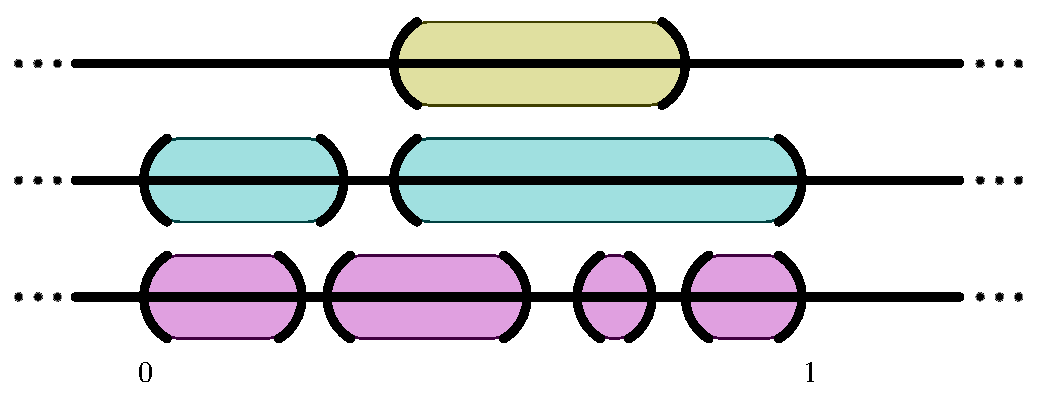
\includegraphics[height=3.285cm]{Figures/2Chapter/lineintervals}
\end{psfrags}
\end{center}

Specifically, for constants $0 \leq a_1 < b_1 < a_2 < b_2 < \cdots \leq 1$, we get
\begin{equation*}
\Pr \left( \bigcup_{k=1}^{\infty} (a_k,b_k) \right)
= \sum_{k=1}^{\infty} b_k - a_k .
\end{equation*}
The probabilities of more complex events can be obtained by considering additional elementary set operations.
However, it suffices to say for now that specifying the probability of the outcome falling in $(a,b)$ for every possible open interval is enough to define a probability law on $\Omega$.
In the example at hand, \eqref{equation:DefinitionProbabilityLaw1} completely determines the probability law on $[0,1]$.

Note that we can give an alternative means of computing the probability of an interval.
Again, consider the open interval $(a, b)$ where $0 \leq a < b \leq 1$.
The probability of the outcome falling in this  interval is equal to
\begin{equation*}
\Pr ( (a, b) ) = b - a = \int_a^b dx = \int_{(a,b)} dx .
\end{equation*}
Moreover, for $0 \leq a_1 < b_1 < a_2 < b_2 < \cdots \leq 1$, we can write
\begin{equation*}
\Pr \left( \bigcup_{k=1}^{\infty} (a_k,b_k) \right)
= \sum_{k=1}^{\infty} \left( b_k - a_k \right)
= \int_{\bigcup_{k=1}^{\infty} (a_k,b_k)} dx .
\end{equation*}
For this carefully crafted example, it appears that the probability of an admissible event $A$ is given by the integral
\begin{equation*}
\Pr (A) = \int_{A} dx .
\end{equation*}
This is indeed accurate for the experiment at hand.
In fact, the class of admissible events for this experiment is simply the collection of all sets for which the integral $\int_A dx$ can be computed.
In other words, if a number is chosen at random from $[0,1]$, then the probability of this number falling in the measurable set $A \subset [0,1]$ is
\begin{equation*}
\Pr (A) = \int_{A} dx .
\end{equation*}
In this document, we will see many probabilistic models with uncountably infinite sample spaces.
The mathematical tools required to handle such models will be treated alongside.

\begin{example}
Suppose that a participant at a game-show is required to spin the wheel of misfortune, a perfect circle with unit circumference.
When subjected to a vigorous spin, the wheel is equally likely to stop anywhere along its periphery.
The sampling space for this experiment is $[0, 1)$, an uncountable set.
Its probability is given by $\Pr ([0, 1)) = 1$.

\begin{center}
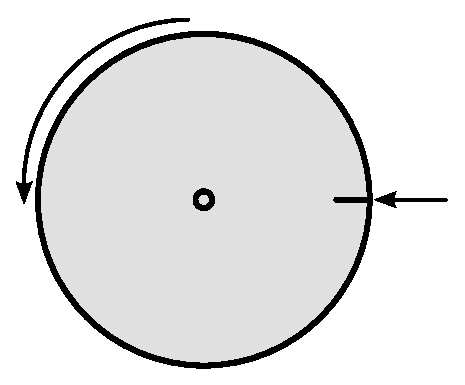
\includegraphics[height=3.15cm]{Figures/2Chapter/wheel}
\end{center}

The probability that the wheel stops in the first quadrant is given by
\begin{equation*}
\Pr \left( \left[ 0, \frac{1}{4} \right) \right) = \frac{1}{4}.
\end{equation*}
Similarly, the probability that the wheel stops in an interval $(a, b)$ where $0 \leq a \leq b < 1$ is
\begin{equation*}
\Pr ((a,b)) = b - a.
\end{equation*}
If $B \subset [0, 1)$ is the measurable set representing a winning outcome, then the probability of success at the wheel is
\begin{equation*}
\Pr(B) = \int_B dy .
\end{equation*}
\end{example}


\subsection{Probability and Measure Theory*}

A systematic treatment of probability involves advanced mathematical concepts.
The basis of our intuition for the infinite is the set of natural numbers,
\begin{equation*}
\NaturalNumbers = \{ 1, 2, \ldots \}.
\end{equation*}
Two sets are said to have the same \emph{cardinality} if their elements can be put in one-to-one correspondence. \index{Cardinality}
A set with the same cardinality as the natural numbers is said to be \emph{countable}. \index{Countable}
That is, the elements of a countable set can always be listed in sequence
\begin{equation*}
s_1, s_2, \ldots
\end{equation*}
although the order may have nothing to do with any relation between the elements.
The integers and the rational numbers are examples of countably infinite sets.
It may be surprising at first to learn that there exist uncountable sets.
To escape beyond the countable, one needs set theoretic tools such as \emph{power sets}. \index{Power set}
The set of real numbers is uncountably infinite; it cannot be put in one-to-one correspondence with the natural numbers.
A typical progression in analysis consists of using the finite to get at the countably infinite, and then to use the countably infinite to get at the uncountable.

It is tempting to try to assign probabilities to every subset of a sample space $\Omega$.
However, for uncountably infinite sample spaces, this leads to serious difficulties that cannot be resolved.
In general, it is necessary to work with special subclasses of the class of all subsets of a sample space $\Omega$.
The collections of the appropriate kinds are called fields and $\sigma$-fields, and they are defined and studied in \emph{measure theory}. \index{Measure theory}
This leads to measure-theoretic probability, and to its unified treatment of the discrete and the continuous.
Fortunately, it is possible to develop an intuitive and working understanding of probability without worrying about these issues.
At some point of your academic career, you may wish to study analysis and measure theory more carefully and in greater details.
However, it is not our current purpose to initiate the study of these fields.

